% Asset ID: FA22GameTheoryEnrichmentTikZ-001
% Source: Transcript graphical method for two expected winnings lines
% Core CCEA status: Optional enrichment only
\documentclass[tikz,border=8pt]{standalone}
\usepackage{amsmath}
\usetikzlibrary{arrows.meta}
\definecolor{Canvas}{HTML}{FAF9F6}\definecolor{Ivory}{HTML}{FFFFF0}\definecolor{LineGrey}{HTML}{E5E5EA}\definecolor{AccentGold}{HTML}{C5A059}\definecolor{DeepGold}{HTML}{D4AF37}\definecolor{SoftPink}{HTML}{FBEFEF}\definecolor{MathText}{HTML}{2C2C2E}
\begin{document}
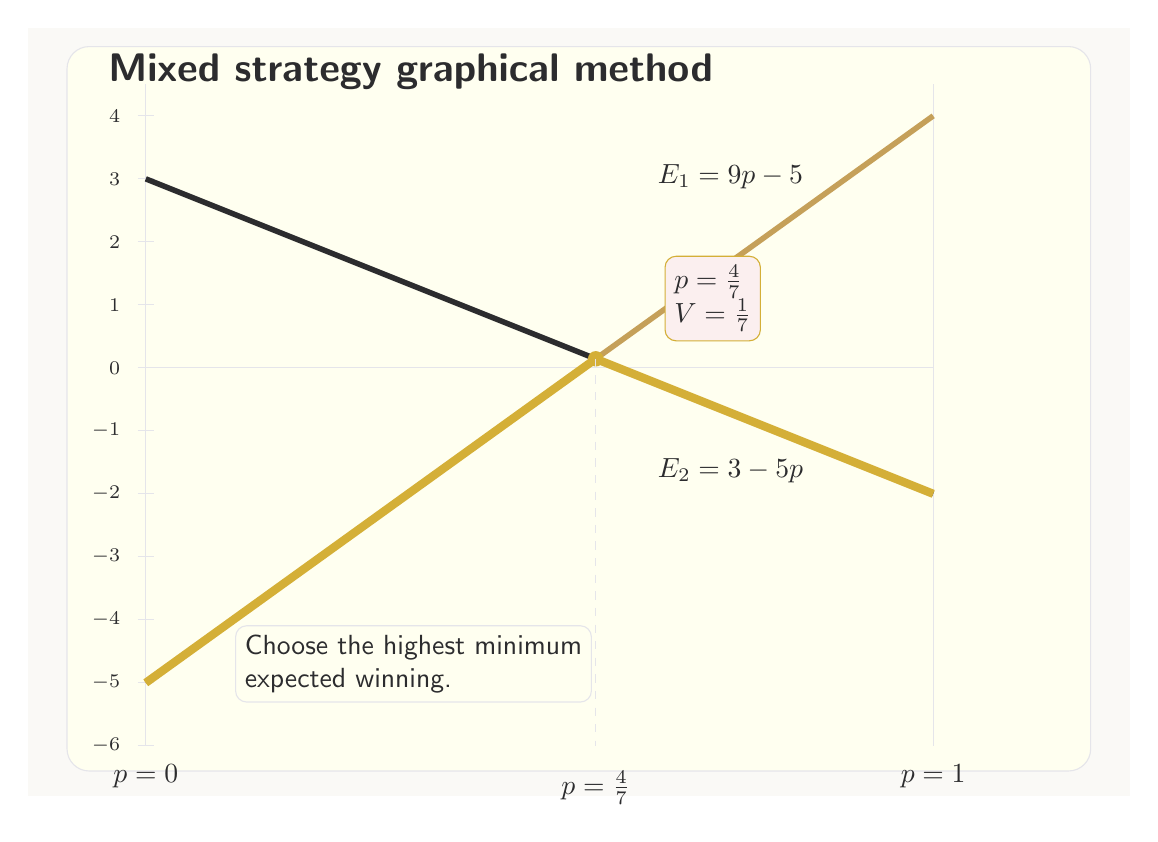
\begin{tikzpicture}[x=10cm,y=0.8cm,>=Latex,every node/.style={font=\sffamily,text=MathText}]
\fill[Canvas] (-.15,-6.8) rectangle (1.25,5.4); \draw[LineGrey,fill=Ivory,rounded corners=8pt] (-.1,-6.4) rectangle (1.2,5.1);
\node[anchor=west,font=\sffamily\bfseries\Large] at (-.06,4.7){Mixed strategy graphical method};
\draw[LineGrey] (0,-6)--(0,4.5); \draw[LineGrey] (1,-6)--(1,4.5); \draw[LineGrey] (0,0)--(1,0);
\foreach \y in {-6,-5,...,4}{\draw[LineGrey] (-.01,\y)--(.01,\y);\node[anchor=east,font=\scriptsize] at (-.02,\y){\(\y\)};}
\draw[AccentGold,line width=2pt] (0,-5)--(1,4) node[pos=.85,above left]{\(E_1=9p-5\)};
\draw[MathText,line width=2pt] (0,3)--(1,-2) node[pos=.85,below left]{\(E_2=3-5p\)};
\coordinate (X) at (0.5714,0.1429); \draw[DeepGold,line width=3pt] (0,-5)--(X)--(1,-2); \fill[DeepGold] (X) circle (2.8pt);
\draw[LineGrey,dashed] (X)--(0.5714,-6); \node[anchor=north] at (0,-6.15){\(p=0\)}; \node[anchor=north] at (1,-6.15){\(p=1\)}; \node[anchor=north] at (0.5714,-6.25){\(p=\frac47\)};
\node[draw=DeepGold,fill=SoftPink,rounded corners=4pt,align=left] at (.72,1.1){\(p=\frac47\)\\ \(V=\frac17\)};
\node[draw=LineGrey,fill=Ivory,rounded corners=4pt,align=left] at (.34,-4.7){Choose the highest minimum\\expected winning.};
\end{tikzpicture}
\end{document}
